% Asset ID: FA21ConicSections2EnrichmentTikZ-001
% Source: horizontal ellipse foci/directrices example
% Boundary status: Off-spec enrichment until official CCEA conics evidence is supplied.
\documentclass[tikz,border=8pt]{standalone}
\usepackage{amsmath,amssymb}
\usetikzlibrary{arrows.meta,calc,positioning}
\definecolor{Canvas}{HTML}{FAF9F6}
\definecolor{Ink}{HTML}{2C2C2E}
\definecolor{Gold}{HTML}{C5A059}
\definecolor{GoldDeep}{HTML}{D4AF37}
\begin{document}
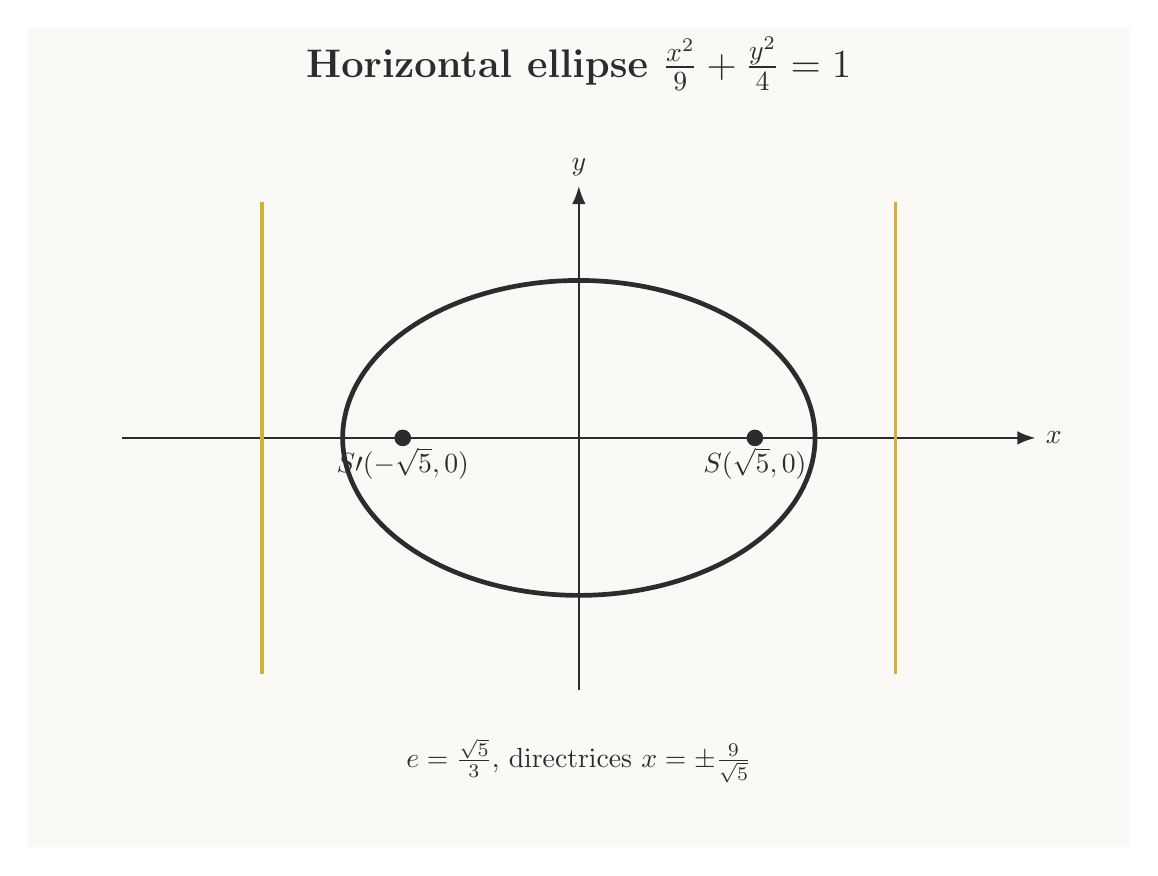
\begin{tikzpicture}[x=1cm,y=1cm,>=Latex]
\fill[Canvas] (-7,-5.2) rectangle (7,5.2);
\node[Ink, font=\Large\bfseries] at (0,4.75) {Horizontal ellipse $\frac{x^2}{9}+\frac{y^2}{4}=1$};
\draw[Ink, thick, -Latex] (-5.8,0)--(5.8,0) node[right] {$x$};\draw[Ink, thick, -Latex] (0,-3.2)--(0,3.2) node[above] {$y$};\draw[GoldDeep, very thick] ({-9/sqrt(5)},-3) -- ({-9/sqrt(5)},3);\draw[GoldDeep, very thick] ({9/sqrt(5)},-3) -- ({9/sqrt(5)},3);\draw[Ink, line width=1.7pt, smooth, samples=240, domain=0:360, variable=\t] plot ({3*cos(\t)}, {2*sin(\t)});\fill[Ink] ({sqrt(5)},0) circle (3pt) node[below] {$S(\sqrt5,0)$};\fill[Ink] ({-sqrt(5)},0) circle (3pt) node[below] {$S\prime(-\sqrt5,0)$};\node[Ink] at (0,-4.1) {$e=\frac{\sqrt5}{3}$, directrices $x=\pm\frac9{\sqrt5}$};
\end{tikzpicture}
\end{document}
